\documentclass[a4paper]{article}
\usepackage{graphicx}
\usepackage{amsmath}
\usepackage{hyperref}
\usepackage{tikz}
\usetikzlibrary{shapes,arrows}
\usepackage{listings}
\lstset{
   basicstyle=\ttfamily,
   mathescape
}

\begin{document}
\title{Graphical models exercises}
\author{Jens Dalgaard Nielsen (Jens.Nielsen@qiagen.com),\\ Patrick Ettenhuber (Patrick.Ettenhuber@qiagen.com)}
\maketitle


\section{Translate graphs into joint probabilities}
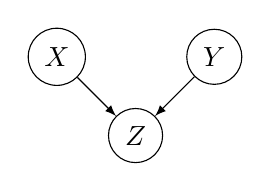
\begin{tikzpicture}%[->,>=stealth',shorten >=1pt,auto,node distance=3cm,
		        %thick,main node/.style={circle,fill=blue!20,draw,minimum size=1cm,inner sep=0pt]}]
                [every path/.style={>=latex},every node/.style={draw,circle}]
  \node            (a) at (0,0)  { $X$ };
  \node            (b) at (2,0)  { $Y$ };
  \node            (c) at (1,-1) { $Z$ };
  \draw[->] (a) edge (c);
  \draw[->] (b) edge (c);
\end{tikzpicture}
$ p(X)p(Y) p(Z|X,Y) $ \\

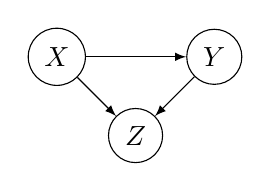
\begin{tikzpicture}%[->,>=stealth',shorten >=1pt,auto,node distance=3cm,
		        %thick,main node/.style={circle,fill=blue!20,draw,minimum size=1cm,inner sep=0pt]}]
                [every path/.style={>=latex},every node/.style={draw,circle}]
  \node            (a) at (0,0)  { $X$ };
  \node            (b) at (2,0)  { $Y$ };
  \node            (c) at (1,-1) { $Z$ };
  \draw[->] (a) edge (c);
  \draw[->] (a) edge (b);
  \draw[->] (b) edge (c);
\end{tikzpicture}
$ p(X)p(Y|X) p(Z|X,Y) $ \\

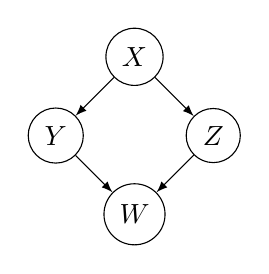
\begin{tikzpicture}%[->,>=stealth',shorten >=1pt,auto,node distance=3cm,
		        %thick,main node/.style={circle,fill=blue!20,draw,minimum size=1cm,inner sep=0pt]}]
                [every path/.style={>=latex},every node/.style={draw,circle}]
  \node            (a) at (0,0)  { $X$ };
  \node            (b) at (-1,-1)  { $Y$ };
  \node            (c) at (1,-1) { $Z$ };
  \node            (d) at (0,-2) { $W$ };
  \draw[->] (a) edge (c);
  \draw[->] (a) edge (b);
  \draw[->] (b) edge (d);
  \draw[->] (c) edge (d);
\end{tikzpicture}
$ p(X)p(Y|X) p(Z|X)p(W|Y,Z) $ \\

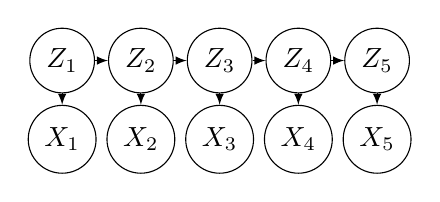
\begin{tikzpicture}%[->,>=stealth',shorten >=1pt,auto,node distance=3cm,
		        %thick,main node/.style={circle,fill=blue!20,draw,minimum size=1cm,inner sep=0pt]}]
                [every path/.style={>=latex},every node/.style={draw,circle}]
  \node            (a) at (0,0)  { $Z_1$ };
  \node            (b) at (0,-1)  { $X_1$ };
  \node            (c) at (1,0)  { $Z_2$ };
  \node            (d) at (1,-1)  { $X_2$ };
  \node            (e) at (2,0)  { $Z_3$ };
  \node            (f) at (2,-1)  { $X_3$ };
  \node            (g) at (3,0)  { $Z_4$ };
  \node            (h) at (3,-1)  { $X_4$ };
  \node            (i) at (4,0)  { $Z_5$ };
  \node            (j) at (4,-1)  { $X_5$ };
  \draw[->] (a) edge (b);
  \draw[->] (a) edge (c);
  \draw[->] (c) edge (d);
  \draw[->] (c) edge (e);
  \draw[->] (e) edge (f);
  \draw[->] (e) edge (g);
  \draw[->] (g) edge (h);
  \draw[->] (g) edge (i);
  \draw[->] (i) edge (j);
\end{tikzpicture}
$ p(Z_1) p(X_1|Z_1)\prod_{i=2}^{5} p(Z_i|Z_{i-1})p(X_i|Z_i)$ \\

\section{Translate joint probabilities into graphs}

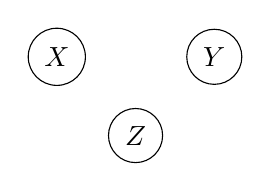
\begin{tikzpicture}%[->,>=stealth',shorten >=1pt,auto,node distance=3cm,
		        %thick,main node/.style={circle,fill=blue!20,draw,minimum size=1cm,inner sep=0pt]}]
                [every path/.style={>=latex},every node/.style={draw,circle}]
  \node            (a) at (0,0)  { $X$ };
  \node            (b) at (2,0)  { $Y$ };
  \node            (c) at (1,-1) { $Z$ };
\end{tikzpicture}
$ p(X)p(Y) p(Z) $ \\

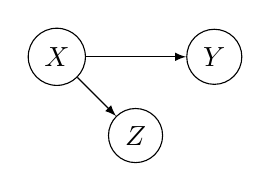
\begin{tikzpicture}%[->,>=stealth',shorten >=1pt,auto,node distance=3cm,
		        %thick,main node/.style={circle,fill=blue!20,draw,minimum size=1cm,inner sep=0pt]}]
                [every path/.style={>=latex},every node/.style={draw,circle}]
  \node            (a) at (0,0)  { $X$ };
  \node            (b) at (2,0)  { $Y$ };
  \node            (c) at (1,-1) { $Z$ };
  \draw[->] (a) edge (c);
  \draw[->] (a) edge (b);
\end{tikzpicture}
$ p(X)p(Y|X) p(Z|X) $ \\

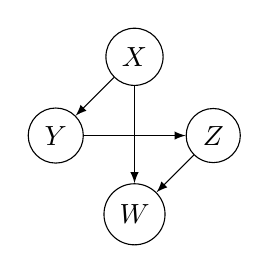
\begin{tikzpicture}%[->,>=stealth',shorten >=1pt,auto,node distance=3cm,
		        %thick,main node/.style={circle,fill=blue!20,draw,minimum size=1cm,inner sep=0pt]}]
                [every path/.style={>=latex},every node/.style={draw,circle}]
  \node            (a) at (0,0)  { $X$ };
  \node            (b) at (-1,-1)  { $Y$ };
  \node            (c) at (1,-1) { $Z$ };
  \node            (d) at (0,-2) { $W$ };
  \draw[->] (a) edge (b);
  \draw[->] (b) edge (c);
  \draw[->] (a) edge (d);
  \draw[->] (c) edge (d);
\end{tikzpicture}
$ p(X)p(Y|X) p(Z|Y)p(W|X,Z) $ \\

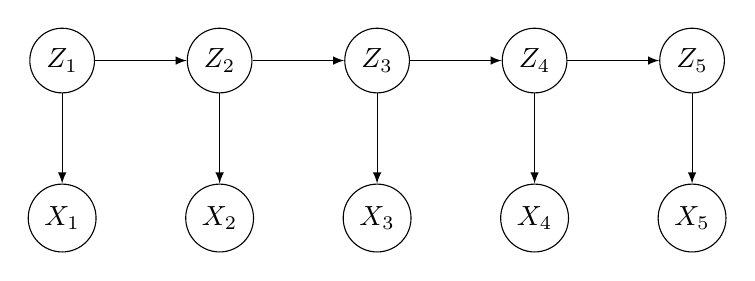
\begin{tikzpicture}%[->,>=stealth',shorten >=1pt,auto,node distance=3cm,
		        %thick,main node/.style={circle,fill=blue!20,draw,minimum size=1cm,inner sep=0pt]}]
                [every path/.style={>=latex},every node/.style={draw,circle}]
  \node            (a) at (0,0)  { $Z_1$ };
  \node            (b) at (0,-2)  { $X_1$ };
  \node            (c) at (2,0)  { $Z_2$ };
  \node            (d) at (2,-2)  { $X_2$ };
  \node            (e) at (4,0)  { $Z_3$ };
  \node            (f) at (4,-2)  { $X_3$ };
  \node            (g) at (6,0)  { $Z_4$ };
  \node            (h) at (6,-2)  { $X_4$ };
  \node            (i) at (8,0)  { $Z_5$ };
  \node            (j) at (8,-2)  { $X_5$ };
  \draw[->] (a) edge (b);
  \draw[->] (a) edge (c);
  \draw[->] (c) edge (d);
  \draw[->] (c) edge (e);
  \draw[->] (e) edge (f);
  \draw[->] (e) edge (g);
  \draw[->] (g) edge (h);
  \draw[->] (g) edge (i);
  \draw[->] (i) edge (j);
\end{tikzpicture}
$ p(Z_1) \prod_{i=1}^5 p(X_i|Z_i)\prod_{i=2}^{5} p(Z_i|Z_{i-1})$ \\

\end{document}
